\documentclass{article}
\usepackage{../header}
\usepackage{datetime2}
\def\Xint#1{\mathchoice
	{\XXint\displaystyle\textstyle{#1}}%
	{\XXint\textstyle\scriptstyle{#1}}%
	{\XXint\scriptstyle\scriptscriptstyle{#1}}%
	{\XXint\scriptscriptstyle\scriptscriptstyle{#1}}%
	\!\int}
\def\XXint#1#2#3{{\setbox0=\hbox{$#1{#2#3}{\int}$ }
		\vcenter{\hbox{$#2#3$ }}\kern-0.6\wd0}}
\def\ddashint{\Xint=}
\def\dashint{\Xint-}
\usepackage[
colorinlistoftodos,
textsize=small,          % Sets the text to the smallest LaTeX font size
textwidth=0.7in        % Sets note width slightly smaller than the 1-inch margin
]{todonotes}
\rhead{Nonlinear Wave Equations}
\om 
\title{Random Exercises}
\author{\me}
\date{Fall 2026}

\begin{document}
	\maketitle
	\fullline 
	\tableofcontents
	\xappto\thefootnote{\relax}
	\footnotetext{Last updated: \today\ at \DTMcurrenttime}
	\halfline 
	\newpage 
	\setlength{\parskip}{0.55em}
	
	\section{Overview}
	
	The following document is a compilation of various calculations, computations, and exercises I completed as part of orals prep. The work here is not meant to be an extensive account of my work, by any means. 
	
\newpage 
\section{Functional and Harmonic Analysis} 
\subsection{Stein \& Shakarchi} 

\begin{prb}{1.1}
	Consider $L^{p} = L^{p}(\mathbb{R}^{d})$ with Lebesgue measure. Let $f_{0}(x) = |x|^{-\alpha}$ if $|x| < 1$, $f_{0}(x) = 0$ for $|x|\geq 1$; also let $f_{\infty}(x) = |x|^{-\alpha}$ if $|x|\geq 1$, $f_{\infty}(x) = 0$ when $|x| < 1$. Show that: \vspace{-0.25cm}
	\begin{enumerate}[itemsep =-2pt,label = (\alph{*})]
		\item $f_{0} \in L^{p}$ if and only if $p\alpha < d$. 
		\item $f_{\infty} \in L^{p}$ if and only if $d < p\alpha$. 
		\item What happens if in the definitions of $f_{0}$ and $f_{\infty}$ we replace $|x|^{-\alpha}$ by $|x|^{-\alpha}/(\log(2/|x|))$ for $|x| < 1$, and $|x|^{-\alpha}$ by $|x|^{-\alpha}/(\log(2|x|))$ for $|x|\geq 1$? 
	\end{enumerate}
\end{prb}
\begin{enumerate}[itemsep =-2pt,label = (\alph{*})]
	\item Let $p \geq 1$, and define $f_{0}(x):\mathbb{R}^{d} \to \mathbb{R}$ to be the measurable function 
	\begin{equation*}
		f_{0}(x) = 
		\begin{cases}
			|x|^{-\alpha}, & |x| < 1 \\
			0, & |x| \geq 1.
		\end{cases}
	\end{equation*}
	Then $f_{0}(x) \in L^{p}$ if and only if $\int_{|x|\leq 1}|f_{0}(x)|^{p}\;dx = \int_{|x|\leq 1}|x|^{-p\alpha}\;dx < \infty$. To evaluate this integral, we will use integration in polar coordinates. Using Theorem 2.49 from Folland, one has 
	\begin{align*}
		\begin{split}
			\int_{|x|\leq 1}\frac{1}{|x|^{p\alpha}}\;dx &= \Gamma(S^{d-1})\cdot \int_{0}^{1}r^{-p\alpha + d - 1}\;dr. 
		\end{split}
	\end{align*}
	By calculus in one dimension, we know that the integral on the right side is finite if and only if $-p\alpha + d - 1 > -1$, which implies $p\alpha < d$. Thus, $f_{0} \in L^{p}$ if and only if $p\alpha < d$. 
	
	\item Define $f_{\infty}(x): \mathbb{R}^{d} \to \mathbb{R}$ to be measurable function
	\begin{equation*}
		f_{\infty}(x) = 
		\begin{cases}
			0, & |x| < 1 \\
			|x|^{-\alpha}, & |x|\geq 1.
		\end{cases}
	\end{equation*}
	Then $f_{\infty}(x) \in L^{p}$ if and only if $\int_{|x|\geq 1}|f_{\infty}(x)|^{p}\;dx = \int_{|x|\geq 1}|x|^{-p\alpha}\;dx < \infty$. Using Theorem 2.49 from Folland, one has 
	\begin{equation*}
		\int_{|x|\geq 1}\frac{1}{|x|^{p\alpha}}\;dx = \Gamma(S^{d-1}) \cdot \int_{1}^{\infty}r^{-p\alpha + d - 1}\;dr. 
	\end{equation*}
	By calculus in one dimension, we know that the integral on the right side is finite if and only if $-p\alpha + d - 1 < -1$, which implies $p\alpha > d$. Thus, $f_{\infty}\in L^{p}$ if and only if $p\alpha > d$. 
	\item Now define $f_{0}(x): \mathbb{R}^{d} \to \mathbb{R}$ to be the modified function 
	\begin{equation*}
		f_{0}(x) = 
		\begin{cases}
			\displaystyle \frac{|x|^{-\alpha}}{\log(2/|x|)}, & |x| < 1 \\
			0, & |x| \geq 1. 
		\end{cases}
	\end{equation*}
	As in (a), $f_{0}(x) \in L^{p}$ if and only if 
	\begin{equation*}
		\int_{0}^{1}\frac{r^{-p\alpha + d - 1}}{\log(2/r)^{p}}\;dr < \infty. 
	\end{equation*}
	Let $k \coloneqq -p\alpha + d - 1$, and define $u = \log(2/r)$. Then the above integral transforms into 
	\begin{align*}
		\begin{split}
			\int_{0}^{1}\frac{r^{-p\alpha + d - 1}}{\log(2/r)^{p}}\;dr &= -\int_{\log(2)}^{\infty}\frac{2^{k}e^{-ku}}{u^{p}}\;(-2e^{-u}\;du) = 2^{k + 1}\int_{\log(2)}^{\infty}\frac{e^{-(k + 1)u}}{u^{p}}\;du. 
		\end{split}
	\end{align*}
	In the limit $u \to \infty$, if $p > 1$, the integrand decays to zero provided $k + 1 \geq 0$. Thus, $f_{0}(x) \in L^{p}$ if and only if $k \geq -1$, which is equivalent to requiring $p\alpha \leq d$. If $p = 1$, then $f_{0}(x) \in L^{p}$ if and only if $p\alpha < d$. Now define the modified function $f_{\infty}(x): \mathbb{R}^{d} \to \mathbb{R}$ by 
	\begin{equation*}
		f_{\infty}(x) = 
		\begin{cases}
			0, & |x| < 1 \\
			\displaystyle\frac{|x|^{-\alpha}}{\log(2|x|)}, & |x| \geq 1. 
		\end{cases}
	\end{equation*}
	As in (b), $f_{\infty}(x) \in L^{p}$ if and only if the integral 
	\begin{equation*}
		\int_{1}^{\infty}\frac{r^{-p\alpha + d - 1}}{\log(2r)}\;dr < \infty. 
	\end{equation*}
	Taking $u = \log(2r)$ this time, the above integral transforms into 
	\begin{align*}
		\begin{split}
			\int_{1}^{\infty}\frac{r^{-p\alpha + d - 1}}{\log(2r)^{p}}\;dr &= \int_{\log(2)}^{\infty}\frac{2^{-k}e^{ku}}{u^{p}}(2^{-1}e^{u}\;du) = 2^{-(k + 1)}\int_{\log(2)}^{\infty}\frac{e^{(k + 1)u}}{u^{p}}\;du. 
		\end{split}
	\end{align*}
	Here, we must consider two cases. First, suppose $p > 1$. Then the integrand decays to zero provided $k + 1 \leq 0$ (corresponding to $p\alpha \geq d$). Thus $f_{\infty}(x) \in L^{p}$ for $p > 1$ if and only if $p\alpha \geq d$. On the other hand, if $p = 1$, then the integral is finite if and only if $k + 1 \lneq 0$, which corresponds to $p\alpha < d$. Thus, 
	\begin{equation*}
		f_{\infty}(x) \in L^{p}(\mathbb{R}^{d}) \text{ if and only if }
		\begin{cases}
			p\alpha \geq d, & p > 1 \\
			\alpha > d, & p = 1.
		\end{cases}
	\end{equation*}
\end{enumerate}

\begin{prb}{1.8}
	Suppose $1 \leq p < \infty$, and that $\mathbb{R}^{d}$ is equipped with Lebesgue measure. Show that if $f \in L^{p}(\mathbb{R}^{d})$, then 
	\begin{equation*}
		\norm{f(x + h) - f(x)}_{L^{p}} \to 0 \quad \text{ as $|h| \to 0$}. 
	\end{equation*}
	Prove that this fails when $p = \infty$. 
	
	[Hint: By the previous exercise, the continuous functions with compact support are dense in $L^{p}(\mathbb{R}^{d})$ for $1 \leq p < \infty$.]
\end{prb}

Fix $1\leq p < \infty$, and assume that $\mathbb{R}^{d}$ is equipped with Lebesgue measure. Further fix some $f \in L^{p}(\mathbb{R}^{d})$. By the density of $C_{c}(\mathbb{R}^{d})$ in $L^{p}(\mathbb{R}^{d})$, there exists a sequence $\{g_{j}\}_{j = 1}^{\infty}$ of compactly supported continuous functions so that $g_{j} \to f$ under the $L^{p}$-norm. First, we will show that for every $j$, $\norm{g_{j}(h + \cdot) - g_{j}}_{p} \to 0$ as $h \to 0$. Without loss of generality, let $|h| \leq R$ for some $R > 0$. Then by continuity of $g_{j}$, $|g_{j}(x + h) - g_{j}(x)|^{p} \to 0$ pointwise a.e. as $|h| \to 0$. On the other hand, by continuity of $g_{j}$ and the extreme value theorem, one has 
\begin{equation*}
	|g_{j}(x + h) - g_{j}(x)|^{p} \leq 2^{p-1}(|g_{j}(x + h)|^{p} + |g_{j}(x)|^{p}) \leq M\chi_{K + B_{R}(0)} \in L^{1}(\mathbb{R}^{d}),
\end{equation*}
where $M \eqqcolon 2^{p} \cdot (\max_{K}|g_{j}(x)|)^{p}$. Thus, by the Dominated Convergence Theorem, 
\begin{equation*}
	\int_{\mathbb{R}^{d}}|g_{j}(x + h) - g_{j}(x)|^{p}\;dx \xrightarrow{|h| \to 0} 0. 
\end{equation*}


Now fix $\epsilon > 0$, $j$ large enough so that $\norm{f - g_{j}}_{p}^{p} < \epsilon/3$, and let $\delta > 0$ so that for all $|h| < \delta$, one has $\norm{g_{j}(h + \cdot) - g_{j}}_{p}^{p} < \epsilon/3$. Then we observe that 
\begin{align*}
	\begin{split}
		\norm{f(h + \cdot) - f}_{p}^{p} &= \int_{\mathbb{R}^{d}}|f(x + h) - f(x)|^{p}\;dx \\
		&\hspace{-0.3cm}\leq C\cdot \left[\int_{\mathbb{R}^{d}}|f(x + h) - g_{j}(x + h)|^{p}\;dx + \int_{\mathbb{R}^{d}}|g_{j}(x + h) - g_{j}(x)|^{p}\;dx+ \int_{\mathbb{R}^{d}}|g_{j}(x) - f(x)|^{p}\;dx\right] \\
		&= 2C\norm{f - g_{j}}_{p}^{p} + C \cdot \norm{g_{j}(h + \cdot) - g_{j}}_{p}^{p} \\
		&< C\epsilon. 
	\end{split}
\end{align*}
where in going from the second to the third line, we used translation invariance of the $L^{p}$ norms. Since the left side is independent of $\epsilon$, taking the limit $\epsilon \to 0$ shows that $\norm{f(h + \cdot) - f}_{p}^{p} \to 0$ as $|h| \to 0$. 

Now consider the case of $p = \infty$. Let $f \in L^{\infty}(\mathbb{R}^{d})$ be the following function: 
\begin{equation*}
	f(x) = 
	\begin{cases}
		1, & |x| \geq 1 \\
		-1, & |x| < 1. 
	\end{cases}
\end{equation*}
Then for any $|h| > 0$, one has that $\norm{f(h + \cdot) - f}_{L^\infty} = 2$ so that this norm cannot converge to zero. 

\begin{prb}{1.12}
	Suppose the measure space $(X, \mu)$ is separable as defined in Exercise 10. Let $1 \leq p < \infty$ and $1/p + 1/q = 1$. A sequence $\{f_{n}\}$ with $f_{n} \in L^p$ is said to converge to $f \in L^p$ \textbf{weakly} if 
	\begin{equation*}
		\int f_{n}g\;d\mu \to \int fg\;d\mu \qquad \text{for every $g \in L^q$}. 
	\end{equation*}
	\begin{enumerate}[itemsep =-2pt,label = (\alph{*})]
		\item Verify that if $\norm{f - f_{n}}_{L^p} \to 0$, then $f_{n}$ converges to $f$ weakly. 
		\item Suppose $\sup_{n}\norm{f_{n}}_{L^p} < \infty$. Then, to verify weak convergence, it suffices to check the above convergence for a dense subset of functions $g$ in $L^q$. 
		\item Suppose $1 < p < \infty$. Show that if $\sup_{n}\norm{f_{n}}_{L^p} <\infty$, then there exists $f \in L^p$ and a subsequence $\{n_{k}\}$ so that $f_{n_{k}}$ converges weakly to $f$. 
	\end{enumerate}
\end{prb}
\begin{enumerate}[itemsep =-2pt,label = (\alph{*})]
	\item Assume that $\norm{f - f_{n}}_{L^p} \to 0$. Fix an arbitrary $g \in L^q$. Then by H\"older's inequality, 
	\begin{equation*}
		\abs{\int f_{n}g\;d\mu - \int fg\;d\mu} \leq \int |f_{n} - f||g|\;d\mu \leq \norm{f_{n} - f}_{p}\norm{g}_{q} \xrightarrow{n \to 0} 0. 
	\end{equation*}
	Since $g \in L^q$ was arbitrary, we conclude that $f_{n}$ converges to $f$ weakly. 
	
	\item Suppose $\sup_{n}\norm{f_{n}}_{L^p} < \infty$, and further assume that the above result holds for some dense subset $\mathcal{A}$ in $L^{q}$. Fix an arbitrary $g \in L^q$, and let $\{g_{j}\}_{j = 1}^{\infty} \subset \mathcal{A}$ so that $\norm{g - g_{j}}_{q} \to 0$ as $j \to \infty$. Then 
	\begin{align*}
		\begin{split}
			\abs{\int f_{n}g - \int fg} &= \abs{\int f_{n}g - \int f_{n}g_{j} + \int f_{n}g_{j} - \int fg_{j} + \int fg_{j} - \int fg} \\
			&\leq \int |f_{n}||g - g_{j}| + \abs{\int f_{n}g_{j} - \int fg_{j}} + \int |f||g - g_{j}|\\
			&\leq \norm{f_{n}}_{L^p}\norm{g - g_{j}}_{L^q} + \abs{\int f_{n}g_{j} - \int fg_{j}} + \norm{f}_{L^p}\norm{g - g_{j}}_{L^q} \\
			&\leq \sup_{n}\norm{f_{n}}_{L^p} \norm{g - g_{j}}_{L^p} + \abs{\int f_{n}g_{j} - \int fg_{j}} + \norm{f}_{L^p}\norm{g - g_{j}}_{L^q}. 
		\end{split}
	\end{align*}
	Thus, taking the limit $n \to \infty$ on both sides, and using the fact that for each $j$, the second term vanishes under the limit by hypothesis, one has 
	\begin{equation*}
		\lim_{n \to \infty}\abs{\int f_{n}g -\int fg} \leq \sup_{n}\norm{f_{n}}_{L^p}\norm{g - g_{j}}_{L^p} + \norm{f}_{L^p}\norm{g - g_{j}}_{L^q}. 
	\end{equation*}
	Taking the limit $j \to \infty$ shows that $\int f_{n}g \to \int fg$ so that $f_{n}$ converges to $f$ weakly. 
	\item Suppose $1 < p < \infty$, and assume $\sup_{n}\norm{f_{n}}_{L^p} < \infty$. First, since $X$ was assumed to be separable, then by Exercise 10(b), one has that $L^q(X,\mu)$ is separable. So let $\{g_{j}\}_{j = 1}^{\infty} \subset L^{q}(X,\mu)$ be a countable dense collection. We consider the sequence $\{\int f_{n}g_{1}\;d\mu\}_{n = 1}^{\infty} \subset \mathbb{R}$. First, it follows that this sequence is uniformly bounded: for every $n$, 
	\begin{equation*}
		\abs{\int f_{n}g\;d\mu} \leq \int |f_{n}\|g|\;d\mu \leq \norm{f_{n}}_{L^p}\norm{g}_{L^q} \leq \sup_{n}\norm{f_{n}}_{L^p}\norm{g}_{L^q} < \infty. 
	\end{equation*}
	Thus there exists a subsequence $\{f^{(1)}_{n_{k}}\}_{k = 1}^{\infty}$ so that $\{\int f_{n_{k}}^{(1)}g_{1}\;d\mu\}_{k = 1}^{\infty}$ converges. Now consider the sequence $\{\int f_{n_{k}}^{(1)}g_{2}\;d\mu\}_{k = 1}^{\infty}$. As before, this sequence is uniformly bounded so that there exists a further subsequence $\{f_{n_{k}}^{(2)}\}_{k = 1}^{\infty}$ such that $\{\int f_{n_{k}}^{(2)}g_{2}\}_{k = 1}^{\infty}$ converges. By construction, $\{\int f_{n_{k}}^{(2)}g_{1}\}$ also converges. In this manner, for each $j$, we can obtain a subsequence $\{f_{n_{k}}^{(j)}\}$ so that $\{\int f_{n_{k}}^{(j)}g_{l}\}_{k = 1}^{\infty}$ converges for all $\ell \leq j$. Now construct the sequence $\{f_{n_{k}}\}_{k = 1}^{\infty} = \{f_{n_{j}}^{(j)}\}_{j = 1}^{\infty}$. By construction, $\{\int f_{n_{k}}g_{j}\}_{k = 1}^{\infty}$ converges for all $j$. Now we claim that $\{\int f_{n_{k}}g\}_{k =1}^{\infty}$ converges for all $g \in L^{q}$. Let $\epsilon > 0$ be fixed, $M \coloneqq \sup_{n}\norm{f_{n}}_{L^p} < \infty$, $j$ large enough so that $\norm{g - g_{j}}_{L^q} < \epsilon/(3M)$, and $N$ large enough so that for all $k,m \geq N$, $|\int f_{n_{k}}g_{j} - \int f_{n_{m}}g_{j}| < \epsilon/3$. Then for all $k, m \geq N$, one has 
	\begin{align*}
		\begin{split}
			\abs{\int f_{n_{k}}g - \int f_{n_{m}}g} &\leq 2\sup_{n}\norm{f_{n}}_{L^p}\cdot \norm{g - g_{j}}_{L^q} + \abs{\int f_{n_{k}}g_{j} - \int f_{n_{m}}g_{j}} \\
			&< \frac{2\epsilon}{3} + \frac{\epsilon}{3} = \epsilon. 
		\end{split}
	\end{align*}
	Thus taking $\epsilon \to 0$ concludes the proof of the above claim. Now define the linear functional $T: L^{q} \to\mathbb{R}$ as follows: for any $g \in L^q$, let 
	\begin{equation*}
		T(g) \coloneqq \lim_{n_{j} \to \infty}\int f_{n_{j}}g. 
	\end{equation*}
	It is straightforward to see that this funtional is bounded. Thus since $1 < p, q < \infty$ and $p,q$ are conjugates, by the Riesz Representation Theorem, there exists a unique $f \in L^p$ so that 
	\begin{equation*}
		\int fg = T(g) = \lim_{n_{j} \to \infty}\int f_{n_{j}}g \qquad \quad (g \in L^q(X,\mu)). 
	\end{equation*}
	Thus the proof concludes. 
\end{enumerate}

\begin{prb}{2.2}
	The following are simple generalizations of the Hausdorff-Young inequalities. \vspace{-0.25cm} 
	\begin{enumerate}[itemsep =-2pt,label = (\alph{*})]
		\item Suppose $\{\varphi_{n}\}$ is an orthonormal sequence on $L^{2}(X, \mu)$. Assume also that $|\varphi_{n}(x)| \leq M$ for all $n$. If $a_{n} = \int f\bar{\varphi}_{n}\;d\mu$, then $\norm{a_{n}}_{L^{q}} \leq M^{(2/p) - 1}\norm{f}_{L^{p}(X)}$, $1 \leq p \leq 2$, $1/p + 1/q = 1$. 
		\item Suppose $f \in L^{p}$ on the torus $\mathbb{T}^{d}$, and $a_{n}= \int_{\mathbb{T}^{d}}f(x)e^{-2\pi i n \cdot x}\;dx$, $n \in \mathbb{Z}^{d}$. Then $\norm{\{a_{n}\}}_{L^{q}(\mathbb{Z}^{d})} \leq \norm{f}_{L^{p}(\mathbb{T}^{d})}$, where $1/q \leq 1 - 1/p$. 
	\end{enumerate}
\end{prb}
\begin{enumerate}[itemsep =-2pt,label = (\alph{*})]
	\item We initially define the operator $T$ on simple functions $f$ by $Tf = \{a_{n}\}$, where 
	\begin{equation*}
		a_{n} \coloneqq \int f\bar{\varphi}_{n}\;d\mu. 
	\end{equation*}
	Then clearly, for $(p_{0},q_{0})= (1,\infty)$, one has that since for each $n$, 
	\begin{equation*}
		|a_{n}| \leq \int |f||\bar{\varphi}_{n}|\;d\mu \leq \int M|f| = M\norm{f}_{L^{1}(X)}, 
	\end{equation*}
	$\norm{a_{n}}_{L^{\infty}} = \sup|a_{n}| \leq M\norm{f}_{L^{1}(X)}$. Thus by Proposition 5.4, we conclude that there exists a unique extension $T$ to all of $L^{1}(X)$ satisfying the same bound. Likewise, for $(p_{1}, q_{1}) = (2, 2)$ and any simple function $f$, Bessel's inequality implies that 
	\begin{equation*}
		\norm{a_{n}}_{L^{2}} = \left(\sum_{n = 1}^{\infty}|a_{n}|^{2}\right)^{1/2} \leq \norm{f}_{L^{2}(X)} = M^{\frac{2}{2} - 1}\norm{f}_{L^{2}(X)}. 
	\end{equation*}	
	Thus by Proposition 5.4, there exists a unique extension $T$ to all of $L^{2}(X)$ satisfying the same bound. Then, the Riesz-Thorin Interpolation Theorem tells us that $\norm{a_{n}}_{L^{q}} \leq M \norm{f}_{L^{p}(X)}$ where 
	\begin{equation*}
		\frac{1}{p} = \frac{1 - t}{p_{0}} + \frac{t}{p_{1}} = 1 - \frac{1}{2}t, \qquad \frac{1}{q} = \frac{1 - t}{q_{0}} + \frac{t}{q_{1}} = \frac{1}{2}t, 
	\end{equation*} 
	where $t \in [0,1]$ (thus corresponding to $1 \leq p \leq 2$, $p^{-1} + q^{-1} = 1$), and where 
	\begin{equation*}
		M \leq M^{1 - t} = M^{2(1 - (1/2)t) - 1} = M^{\frac{2}{p} - 1}. 
	\end{equation*}
	\item As before, initially define the operator $T$ on simple functions $f$ on $\mathbb{T}^{d}$ by $Tf = \{a_{n}\}$, where for each $n \in \mathbb{Z}^{d}$, 
	\begin{equation*}
		a_{n} \coloneqq \int_{\mathbb{T}^{d}}f(x)e^{-2\pi i n \cdot x}\;dx. 
	\end{equation*} 
	Clearly for $(p_{0}, q_{0}) = (1, \infty)$, one has 
	\begin{equation*} 
		|a_{n}| \leq \int_{\mathbb{T}^{d}}|f(x)| = \norm{f}_{L^{1}(\mathbb{T}^{d})}, 
	\end{equation*} 
	so that 
	\begin{equation*}
		\norm{\{a_{n}\}}_{L^{\infty}(\mathbb{Z}^{d})} = \sup_{n}|a_{n}| \leq \norm{f}_{L^{1}(\mathbb{T}^{d})}. 
	\end{equation*} 
	Thus Proposition 5.4 gives a unique extension of $T$ to all $L^{1}(\mathbb{T}^{d})$ that satisfies the same bound. Now consider $(p_{1}, q_{1}) = (\infty, \infty)$. Then for any $n \in \mathbb{Z}^{d}$, one has that 
	\begin{equation*}
		|a_{n}| \leq \int_{\mathbb{T}^{d}}|f(x)| \leq \norm{f}_{L^{\infty}(\mathbb{T}^{d})}, 
	\end{equation*}
	where we assume that $dx$ denotes the normalized measure on $\mathbb{T}^{d}$. Thus taking the supremum over all $n \in \mathbb{Z}^{d}$, and using Proposition 5.4 concludes the claim. Likewise, one can show this property holds for the pair $(p_{2},q_{2}) = (2, 2)$. Since $\mathbb{T}^{d}$ has finite measure, it follows that for all $p \geq 2$ (i.e., $1/p \leq 1/2$), $L^{p}(\mathbb{T}^{d}) \hookrightarrow L^{2}(\mathbb{T}^{d})$. Thus, using Proposition 5.4, we also get the endpoint $(p_{3},q_{3}) = (p, 2)$ for all $p \geq 2$. The Riesz diagram as of now is given by 
	\begin{figure}[h!]
		\centering 
		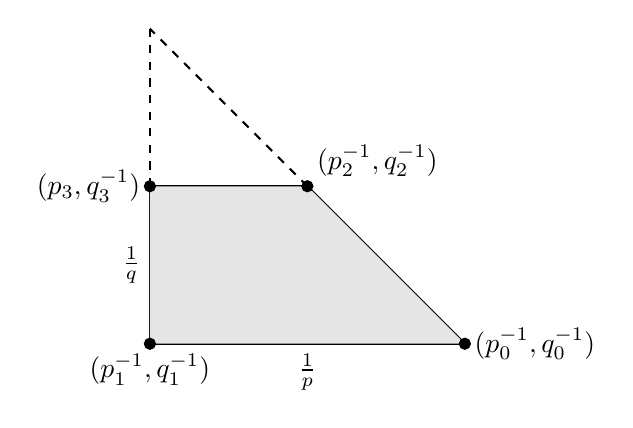
\begin{tikzpicture} 
			\draw[thick] (0,0) -- (4,0); \draw[thick] (0,0) -- (0,2); 
			\draw[thick, dashed] (0,2) -- (0,4); 
			\draw[thick] (4,0) -- (2,2); \draw[thick,dashed] (2,2) -- (0,4); 
			\draw[thick] (0,2) -- (2,2); 
			\fill[black!10] (0,0) -- (4,0) -- (2,2) -- (0,2) -- cycle;
			\draw (2,0) node[anchor =north] {$\frac{1}{p}$}; \draw (0,1) node[anchor=east] {$\frac{1}{q}$}; 
			\draw[fill=black] (2,2) circle(2pt) node[anchor = south west] {$(p_{2}^{-1}, q_{2}^{-1})$}; 
			\draw[fill=black] (4,0) circle(2pt)node[anchor = west] {$(p_{0}^{-1}, q_{0}^{-1})$}; 
			\draw[fill=black] (0,0) circle(2pt) node[anchor = north] {$(p_{1}^{-1}, q_{1}^{-1})$}; 
			\draw[fill=black] (0,2) circle(2pt) node[anchor = east] {$(p_{3}, q_{3}^{-1})$}; 
		\end{tikzpicture}
	\end{figure}
\end{enumerate}

\begin{prb}{2.3}
	Check that an inequality of the form $\norm{\hat{f}}_{L^{q}(\mathbb{R}^{d})} \leq A \norm{f}_{L^{p}(\mathbb{R}^{d})}$ (holding for all simple functions $f$) is possible if and only if $1/p + 1/q = 1$. \newline [Hint: Let $f_{r}(x) = f(rx)$, $r > 0$. Then $\hat{f}_{r}(\xi) = \hat{f}(\xi/r)r^{-d}$.]
\end{prb}
Let $f$ be an arbitrary fixed simple function. As suggested by the hint, let $r > 0$, and define $f_{r}(x) = f(rx)$ so that $\hat{f}_{r}(\xi) = \hat{f}(\xi/r)r^{-d}$. We note that $f_{r}$ is also a simple function. We now compute, 
\begin{align*}
	\begin{split}
		\norm{\hat{f}_{r}}_{L^{q}(\mathbb{R}^{d})} &= \left(\int_{\mathbb{R}^{d}}|\hat{f}(\xi/r)|^{q}r^{-dq}\;d\xi\right)^{1/q} \\
		&= r^{-d}\left(\int_{\mathbb{R}^{d}}|\hat{f}(\xi/r)|^{q}\;d\xi\right)^{1/q} \\
		&= r^{-d}\left(\int_{\mathbb{R}^{d}}|\hat{f}(\eta)|^{q}r^{d}\;d\eta\right)^{1/q} \\
		&= r^{d(-1 + 1/q)}\norm{\hat{f}}_{L^{q}(\mathbb{R}^{d})}. 
	\end{split} 
\end{align*}
Likewise, 
\begin{align*}
	\begin{split}
		\norm{f_{r}}_{L^{p}(\mathbb{R}^{d})} &= \left(\int_{\mathbb{R}^{d}}|f(rx)|^{p}\;dx\right)^{1/p} \\
		&= \left(\int_{\mathbb{R}^{d}}|f(y)|r^{-d}\;dy\right)^{1/p} = r^{-d/p}\norm{f}_{L^{p}(\mathbb{R}^{d})}. 
	\end{split} 
\end{align*}
So we have the following: the above estimate holds for all simple functions $f$ if and only if for any $r > 0$, 
\begin{equation*}
	\norm{\hat{f}_{r}}_{L^{q}(\mathbb{R}^{d})} \leq A \norm{f}_{L^{p}(\mathbb{R}^{d})} \quad \text{and} \quad \norm{\hat{f}}_{L^{q}(\mathbb{R}^{d})} \leq A\norm{f}_{L^{p}(\mathbb{R}^{d})}. 
\end{equation*} 
But our work above shows that the first inequality is equivalent to the estimate 
\begin{equation*}
	r^{-d + d/q}\norm{\hat{f}}_{L^{q}(\mathbb{R}^{d})} \leq r^{-d/p}\norm{f}_{L^{p}(\mathbb{R}^{d})} \iff \norm{\hat{f}}_{L^{q}(\mathbb{R}^{d})} \leq r^{d(1 - 1/q - 1/p)}A\norm{f}_{L^{q}(\mathbb{R}^{d})}. 
\end{equation*}
Thus since $r > 0$ is arbitrary, the above estimate is consistent with the two inequality we have above if and only if $1 - 1/q - 1/p = 0$ iff $1/q + 1/p = 1$. 

\begin{prb}{2.10}
	Suppose $f \in L^{p}(\mathbb{R})$. Verify that: \vspace{-0.25cm}
	\begin{enumerate}[itemsep =-2pt,label = (\alph{*})]
		\item $\norm{f \ast \mathcal{P}_{y}}_{L^{p}(\mathbb{R})} \leq \norm{f}_{L^{p}}$, $1 \leq p \leq \infty$. 
		\item $f \ast \mathcal{P}_{y} \to f$, as $y \to 0$ in the $L^{p}$ norm when $1 \leq L^{p} < \infty$. 
	\end{enumerate}
\end{prb} 
\begin{enumerate}[itemsep =-2pt,label = (\alph{*})]
	\item Let $\mathcal{P}_{y}(x)$ denote the \textbf{Poisson kernel}, 
		\begin{equation*}
			\mathcal{P}_{y}(x) \coloneqq \frac{1}{\pi}\frac{y}{x^{2} + y^{2}}. 
		\end{equation*} 
		Let $p_{0} = 1$, and define the operator $T$ on $L^{p_{0}}(\mathbb{R})$, initially just on the set of all simple functions, by $Tf \coloneqq (f \ast \mathcal{P}_{y})(x)$. First, if $y = 0$, then $P_{y}(x) \equiv 0$ so that $Tf \equiv 0$, and the result holds trivially. So assume $y \neq 0$ (wlog, assume $y > 0$). Then we compute, 
		\begin{align*}
			\begin{split}
				\norm{\mathcal{P}_{y}}_{L^{1}(\mathbb{R})} &= \int_{\mathbb{R}} \frac{1}{\pi}\frac{\abs{y}}{x^{2} + y^{2}}\;dx \\
				&= \frac{1}{\pi}\frac{|y|}{y} \arctan\left(\frac{x}{y}\right)\bigg|_{-\infty}^{\infty} = \frac{1}{\pi}\frac{|y|}{y} \cdot \left[\frac{\pi}{2} + \frac{\pi}{2}\right] = \frac{|y|}{y} =1. 
			\end{split} 
		\end{align*}
		Thus for $p_{0} = 1$, we have 
		\begin{align*}
			\begin{split} 
				\norm{Tf}_{L^{1}(\mathbb{R})} &= \int_{\mathbb{R}}\abs{\frac{1}{\pi}\int_{\mathbb{R}}\frac{f(x - t)y}{y^{2} + t^{2}}\;dt}\;dx \\
				&\leq \int_{\mathbb{R}}\int_{\mathbb{R}}|f(x - t)| \cdot \abs{\frac{1}{\pi}\frac{y}{y^{2} + t^{2}}}\;dx dt \\
				&= \int_{\mathbb{R}}\norm{f(\cdot - t)}_{L^{1}(\mathbb{R})} \cdot \abs{\frac{1}{\pi}\frac{y}{y^{2} + t^{2}}}\;dt  \\
				&= \int_{\mathbb{R}}\norm{f}_{L^{1}(\mathbb{R})} \cdot \abs{\frac{1}{\pi}\frac{y}{y^{2} + t^{2}}}\;dt = \norm{f}_{L^{1}(\mathbb{R})}\norm{\mathcal{P}_{y}}_{L^{1}(\mathbb{R})} = \norm{f}_{L^{1}(\mathbb{R})}, 
			\end{split} 
		\end{align*} 
		where the second line follows from Minkowski's inequality, and the fourth line follows from translation invariance of the $L^{p}$ norms. Thus by Proposition 5.4, $T$ extends to a unique operator on all of $L^{1}(\mathbb{R})$ satisfying the same estimate. Now define the operator $T$ on $L^{p_{1}}(\mathbb{R})$, where $p_{1} =\infty$, initially on just the set of all simple functions by $Tf \coloneqq (f \ast \mathcal{P}_{y})(x)$. As before, the proof is trivial if $y = 0$. So assume $y \neq 0$. Then for each $x$, 
		\begin{align*}
			\begin{split} 
				|Tf(x)| &= \abs{\int_{\mathbb{R}}\frac{1}{\pi}\frac{f(x - t)y}{y^{2} + t^{2}}\;dt} \\
				&\leq \int_{\mathbb{R}}|f(x - t)| \cdot \abs{\frac{1}{\pi}\frac{y}{y^{2} + t^{2}}}\;dt \\
				&\leq \int_{\mathbb{R}}\norm{f(x - \cdot)}_{L^{\infty}(\mathbb{R})} \cdot \abs{\frac{1}{\pi}\frac{y}{t^{2} +  y^{2}}}\;dt  \\
				&= \int_{\mathbb{R}}\norm{f}_{L^{\infty}(\mathbb{R})} \cdot \abs{\frac{1}{\pi} \frac{y}{t^{2} + y^{2}}}\;dt = \norm{f}_{L^{\infty}(\mathbb{R})} \cdot \norm{\mathcal{P}_{y}}_{L^{1}(\mathbb{R})} = \norm{f}_{L^{\infty}(\mathbb{R})}. 
			\end{split} 
		\end{align*} 
		Using Proposition 5.4, the result extends to all of $L^{\infty}(\mathbb{R})$. On the Riesz diagram, we have proven the estimate for the endpoints $(0,0)$ and $(1,1)$. Thus by the Riesz-Thorin interpolation theorem, the theorem follows for all points on the diagonal line connecting these endpoints (i.e., for all $1 \leq p \leq \infty$). 
		\item Now let $1 \leq p < \infty$, and let $\delta > 0$ be fixed. By continuity of translations in $L^{p}(\mathbb{R})$, there exists $\epsilon > 0$ such that $|t| \leq \delta \implies \norm{f( \cdot - t) - f}_{L^{p}(\mathbb{R})} < \epsilon/2$. Thus we compute, 
		\begin{align*}
			\begin{split}
			\norm{f \ast \mathcal{P}_{y} - f}_{L^{p}} &= \left(\int_{\mathbb{R}} \abs{\int_{\mathbb{R}} \frac{1}{\pi}\frac{f(x - t)y}{t^{2} + y^{2}}\;dt - f(x)}^{p}\;dx\right)^{1/p} \\
			&= \left(\int_{\mathbb{R}} \abs{ \int_{\mathbb{R}}[f(x - t) - f(x)] \cdot \frac{1}{\pi}\frac{y}{t^{2} + y^{2}}\;dt }^{p}\;dx \right)^{1/p} \\
			&\leq \int_{\mathbb{R}}\left(\int_{\mathbb{R}}|f(x - t) - f(x)| \cdot \abs{\frac{1}{\pi}\frac{y}{t^{2} + y^{2}}}^{p}\;dx\right)^{1/p}\;dt \\
			&= \int_{\mathbb{R}}\norm{f(\cdot -t) - f}_{L^{p}(\mathbb{R})} \cdot \abs{\frac{1}{\pi}\frac{y}{t^{2} + y^{2}}}\;dt  \\
			&= \int_{|t| \leq \delta} \norm{f(\cdot -t) - f}_{L^{p}(\mathbb{R})} \cdot \abs{\frac{1}{\pi}\frac{y}{t^{2} + y^{2}}}\;dt + \int_{|t| > \delta}\norm{f(\cdot -t) - f}_{L^{p}(\mathbb{R})} \cdot \abs{\frac{1}{\pi}\frac{y}{t^{2} + y^{2}}}\;dt \\
			&\leq \epsilon/2 + 2\norm{f}_{L^{p}(\mathbb{R})} \cdot \int_{|t| > \delta}\abs{\mathcal{P}_{y}(t)}\;dt, 
			\end{split} 
		\end{align*} 
	where the second line follows from $\norm{\mathcal{P}_{y}}_{L^{1}(\mathbb{R})} = 1$ for any $y \in \mathbb{R}$, and the third line follows from Minkowski's inequality. Since $\mathcal{P}_{y}(t) \to 0$ for all $t \neq 0$ in the limit $y \to 0^{+}$, it follows that the second term tends to $0$ in the limit $y \to 0^{+}$. I.e., there exists some $y_{0}$ so that for all $y < y_{0}$, the second term is bounded above by $\epsilon/(2 \norm{f}_{L^{p}(\mathbb{R})})$. Therefore, we conclude that $\norm{f \ast \mathcal{P}_{y_{0}} - f}_{L^{p}(\mathbb{R})} \leq \epsilon$ so that $f \ast \mathcal{P}_{y} \to f$ in the $L^{p}$ norm. 
\end{enumerate} 

\begin{prb}{2.16}
	Prove that the space $\mathbf{H}^{1}_{r}$ is complete as follows. Let $\{f_{n}\}$ be a Cauchy sequence in $\mathbf{H}^{1}_{r}$. Then since $\{f_{n}\}$ is also Cauchy in $L^{1}$, there is an $L^{1}$ function $f$ so that $f = \lim_{n \to \infty}f_{n}$ in the $L^{1}$-norm. Now for an appropriate subsequence $\{n_{k}\}$, write $f = f_{n_{1}} + \sum_{k = 1}^{\infty}(f_{n_{k + 1}} - f_{n_{k}})$. 
\end{prb}
Let $\mathbf{H}^{1}_{r}$ denote the Hardy space, and let $\{f_{n}\} \subset \mathbf{H}^{1}_{r}$ be a Cauchy sequence. First, we begin by showing that each $f \in L^{1}$. Let $\sum_{j}\lambda_{j}\mathfrak{a}_{j}$ be an arbitrary decomposition of $f$, where each $\mathfrak{a}_{j}$ is an atom, and $\sum |\lambda_{j}| < \infty$. Thus since the sum converges under the $L^{1}$ norm, Fubini/Tonelli implies that 
\begin{equation*}
	\int_{\mathbb{R}}|f|\;dx = \int_{\mathbb{R}}\abs{\sum_{1}^{\infty}\lambda_{k}\mathfrak{a}_{k}} \leq \int_{\mathbb{R}}\sum_{1}^{\infty}|\lambda_{k}||\mathfrak{a}_{k}|= \sum_{1}^{\infty}\int_{\mathbb{R}}|\lambda_{k}||\mathfrak{a}_{k}| = \sum_{1}^{\infty}|\lambda_{k}| < \infty.  
\end{equation*}
Thus since $\sum \lambda_{j}\mathfrak{a}_{j}$ was an arbitrary decomposition of $f$ into a sum of atoms, it follows that $f \in L^{1}$. In particular, taking the infimum over all such decompositions also yields the estimate $\norm{f}_{L^{1}} \leq \norm{f}_{\mathbf{H}^{1}_{r}}$. Thus if $\{f_{n}\}$ is Cauchy in $\mathbf{H}^{1}_{r}$, they are also Cauchy in $L^{1}$. Since the latter is a Banach space, there exists an $L^{1}$ function $f$ such that $f = \lim_{n\to \infty} f_{n}$ in the $L^{1}$-norm. But this implies there exists a subsequence $\{f_{n_{k}}\}$ that converges to $f$ pointwise a.e. Fix $\epsilon > 0$. Since $\{f_{n}\}$ is Cauchy in $\mathbf{H}^{1}_{r}$, for every $k \geq 1$, there exists a positive integer $N_{k}$ such that for all $m, n > N_{k}$, 
\begin{equation*}
	\norm{f_{m} - f_{n}}_{\mathbf{H}^{1}_{r}} < \frac{\epsilon}{2^{k}}. 
\end{equation*} 
Thus from the subsequence $\{f_{n_{k}}\}_{k = 1}^{\infty}$, we construct another subsequence as follows: we choose $n_{1} > N_{1}$. Next, we choose $n_{2} > \max\{n_{1}, N_{2}\}$. Repeating inductively, we obtain a subsequence $\{f_{n_{k}}\}$ such that 
\begin{equation*}
	\sum_{k = 1}^{\infty}\norm{f_{n_{k + 1}} - f_{n_{k}}}_{\mathbf{H}^{1}_{r}} \leq \sum_{k = 1}^{\infty}\frac{\epsilon}{2^{k}} = \epsilon < \infty. 
\end{equation*} 
Now we recall that 
\begin{equation*}
	f = \lim_{j \to\infty}f_{n_{j}} = f_{n_{1}} + \lim_{j \to \infty}\sum_{k = 1}^{j}(f_{n_{k + 1}} - f_{n_{k}}) = f_{n_{1}} + \sum_{1}^{\infty}(f_{n_{k + 1}} - f_{n_{k}}). 
\end{equation*} 
Thus 
\begin{equation*}
	\norm{f}_{\mathbf{H}^{1}_{r}} \leq \norm{f_{n_{1}}}_{\mathbf{H}^{1}_{r}} + \sum_{k = 1}^{\infty}\norm{f_{n_{k + 1}} - f_{n_{k}}}_{\mathbf{H}^{1}_{r}} < \infty, 
\end{equation*}
which estalishes that $f \in \mathbf{H}^{1}_{r}$. All that remains to be shown is that $f_{n} \to f$ under the $\mathbf{H}_{r}^{1}$ norm. We compute, 
\begin{align*}
	\begin{split}
		\norm{f - f_{n}}_{\mathbf{H}^{1}_{r}} &\leq \norm{f - f_{n_{k}}}_{\mathbf{H}^{1}_{r}} + \norm{f_{n_{k}} - f_{n}}_{\mathbf{H}^{1}_{r}}. 
	\end{split} 
\end{align*} 
Since the sequence $\{f_{n}\}$ is Cauchy in $\mathbf{H}^{1}_{r}$, the second term vanishes in the limit $n, k \to \infty$. On the other hand, since 
\begin{equation*}
	\norm{f - f_{n_{k}}}_{\mathbf{H}^{1}_{r}} \leq \sum_{j = k}^{\infty}\norm{f_{n_{k + 1}} - f_{n_{k}}}_{\mathbf{H}^{1}_{r}}. 
\end{equation*} 
By our construction of the subsequence $\{f_{n_{k}}\}$, we can control the sum by $\epsilon$. Thus we conclude that $f_{n} \to f$ under the $\mathbf{H}^{1}_{r}$ norm, which means that $\mathbf{H}^{1}_{r}$ is a Banach space. 

\begin{prb}{2.20}
	When $f \in L^{1}(\mathbb{R}^{d})$ we know that its Fourier transform is bounded and $\hat{f}(\xi)$ tends to $0$ as $|\xi|\to \infty$ (the Riemann-Lebesgue lemma), but no better assertion about the ``smallness'' of $\hat{f}$ can be made. (For the analogous result for Fourier series, see Chapter 3 in Book III.) Show, however, that for $f \in \mathbf{H}^{1}_{r}$ we have 
	\begin{equation*}
		\int_{\mathbb{R}^{d}}|\hat{f}(\xi)|\;\frac{d\xi}{|\xi|^{d}} \leq A \norm{f}_{\mathbf{H}^{1}_{r}}. 
	\end{equation*} 
	[Hint: Verify this for atoms.]
\end{prb} 
First, assume that for every atom $\mathfrak{a}$, the above estimate holds
Then for any decomposition, $f = \sum_{k = 1}^{\infty}\lambda_{k}\mathfrak{a}_{k}$ into atoms, 
\begin{align*}
	\begin{split}
		\int_{\mathbb{R}^{d}}|\hat{f}(\xi)|\;\frac{d\xi}{|\xi|^{d}} &= \int_{\mathbb{R}^{d}}\abs{\sum_{1}^{\infty}\lambda_{k}\hat{\mathfrak{a}}_{k}}\;\frac{d\xi}{|\xi|^{d}} \\
		&\leq \sum_{1}^{\infty}\int_{\mathbb{R}^{d}}|\lambda_{k}||\hat{\mathfrak{a}}_{k}|\;\frac{d\xi}{|\xi|^{d}} \\
		&\leq A\sum_{1}^{\infty}|\lambda_{k}|. 
	\end{split} 
\end{align*} 
Thus taking the infimum over all such decompositions of $f$, we obtain, 
\begin{equation*}
	\int_{\mathbb{R}^{d}}|\hat{f}(\xi)|\;\frac{d\xi}{|\xi|^{d}} \lesssim \norm{f}_{\mathbf{H}^{1}_{r}}. 
\end{equation*}
So now, we will show that the result holds true for every atom. Let $\mathfrak{a}$ be an atom on $\mathbb{R}^{d}$; without loss of generality, we can assume that $\mathfrak{a}$ is supported on the unit ball $B_{1}(0) \subset \mathbb{R}^{d}$. Assume $\mathfrak{a}$ is not identically zero. Then one has that 
\begin{equation*}
	\hat{\mathfrak{a}}(\xi) \coloneqq \int_{\mathbb{R}^{d}}\mathfrak{a}(x)e^{-2\pi i x \cdot \xi}\;dx = \int_{|x| \leq 1}\mathfrak{a}(x)e^{-2\pi i x \cdot \xi}\;dx = \int_{|x| \leq 1}\mathfrak{a}(x)\left(e^{-2\pi i x \cdot \xi} - 1\right)\;dx, 
\end{equation*} 
where the final equality follows from the fact that $\int_{\mathbb{R}^{d}} \mathfrak{a}(x) = 0$. Thus, 
\begin{align*}
	\begin{split}
		\int_{\mathbb{R}^{d}}|\hat{\mathfrak{a}}(\xi)|\;\frac{d\xi}{|\xi|^{d}} &= \int_{|\xi| \leq 1}\abs{\int_{|x| \leq 1}\mathfrak{a}(x)\frac{e^{-2\pi i x \cdot \xi} - 1}{|\xi|^{d}}\;dx}\;d\xi + \int_{|\xi| > 1} |\hat{\mathfrak{a}}(\xi)|\;\frac{d\xi}{|\xi|^{d}} \\
		&\leq \int_{|x| \leq 1}\int_{|\xi| \leq 1}|\mathfrak{a}(x)| \cdot \abs{\frac{e^{-2\pi i x \cdot \xi} - 1}{|\xi|^{d}}}\;d\xi dx + \int_{|\xi| > 1|}|\hat{\mathfrak{a}}(\xi)|\;\frac{d\xi}{|\xi|^{d}} \\
		&\leq 2\pi \norm{\mathfrak{a}}_{L^{1}(\mathbb{R}^{d})} + \left(\int_{|\xi| > 1}|\hat{\mathfrak{a}}(\xi)|^{2}\;d\xi\right)^{1/2}\left(\int_{|\xi| > 1}\frac{1}{|\xi|^{2d}}\;d\xi\right)^{1/2} \\
		&= 2\pi \norm{\mathfrak{a}}_{L^{1}(\mathbb{R}^{d})} + \left(\int_{|x|\leq 1}\abs{\mathfrak{a}(\xi)}^{2}\;dx\right)^{1/2} \\
		&\leq 2\pi \norm{\mathfrak{a}}_{L^{1}(\mathbb{R}^{d})} + \left(\frac{1}{m(B_{1}(0))}\right)^{1/2} \leq 2\pi + \frac{1}{m(B_{1}(0))^{1/2}} \equiv A < \infty. 
	\end{split} 
\end{align*} 

\newpage 

\subsection{Evans} 
\begin{prb}{2.18}
	(Stokes' rule) Assume $u$ solves the initial-value problem 
	\begin{equation*}
		\left\{
		\begin{alignedat}{3}
			u_{tt} - \Delta u &= 0 &\qquad& \text{in $\mathbb{R}^{n} \times (0, \infty)$} \\
			u =0, u_{t} &= h, &\qquad& \text{on $\mathbb{R}^{n} \times \{t = 0\}$}. 
		\end{alignedat}
		\right.
	\end{equation*}
	Show that $v \coloneqq u_{t}$ solves 
	\begin{equation*}
		\left\{
		\begin{alignedat}{3}
			v_{tt} - \Delta v &= 0 &\qquad& \text{in $\mathbb{R}^{n} \times (0, \infty)$} \\
			v =h, v_{t} &= 0, &\qquad& \text{on $\mathbb{R}^{n} \times \{t = 0\}$}. 
		\end{alignedat}
		\right.
	\end{equation*}
	This is \textit{Stokes' rule.}
\end{prb}
Assume $u$ solves the given IVP, and let $v \coloneqq u_{t}$. One immediately notes that on $\mathbb{R}^{n} \times \{t = 0\}$, since $u_{t} = h$, $v = h$. Second, $v_{t} = u_{tt}$. On $\mathbb{R}^{n} \times \{t = 0\}$, $u \equiv 0$ so that $\Delta u = 0$. But since $u$ satisfies the wave equation $u_{tt} = \Delta u \equiv 0$. Thus $v_{t} \equiv 0$ on $\mathbb{R}^{n} \times \{t = 0\}$. Next we note that $\partial_{t}$ and $\partial_{x^{j}}$ commute for any $1 \leq j \leq n$. Thus since $u$ satisfies $u_{tt} - \Delta u = 0$, differentiating both sides by $t$, one obtains 
\begin{equation*}
	u_{ttt} - \Delta u_{t} = 0 \iff v_{tt} - \Delta v = 0 
\end{equation*}
in $\mathbb{R}^{n} \times (0,\infty)$. 

\begin{prb}{2.19}
	$ $\newline \vspace{-0.25cm}
	\begin{enumerate}[itemsep =-2pt,label = (\alph{*})]
		\item Show the general solution of the PDE $u_{xy} = 0$ is 
		\begin{equation*}
			u(x, y) = F(x) + G(y) 
		\end{equation*}
		for arbitrary functions $F, G$. 
		\item Using the change of variables $\xi = x + t$, $\eta = x - t$, show $u_{tt} - u_{xx} = 0$ if and only if $u_{\xi\eta} = 0$. 
		\item Use (a) and (b) to rederive d'Alembert's formula. 
		\item Under what conditions on the initial data $g, h$ is the solution $u$ a right-moving wave? A left-moving wave? 
	\end{enumerate}
\end{prb}
\begin{enumerate}[itemsep =-2pt,label = (\alph{*})]
	\item Consider the PDE $u_{xy} =0$. Let $v(x,y) = u_{x}$. Then $v$ satisfies the differential equation $v_{y} = 0$. Thus since $v$ is independent of $y$, one has $u_{x}(x,y) = v(x,y) = f(x)$ for some arbitrary function $f$. But then integrating both sides with respect to $x$, and supposing that $F(x)$ is the antiderivative of $f(x)$, 
	\begin{equation*}
		u(x,y) = F(x) + G(y), 
	\end{equation*}
	where $G$ is some arbitrary function of $y$. 
	\item Define $\xi = x + t$ and $\eta = x -t$ so that $x = (\xi + \eta)/2$ and $t = (\xi - \eta)/2$. Then, 
	\begin{align*}
		\begin{split}
			u_{\xi} &= u_{x}\frac{\partial x}{\partial \xi} + u_{t}\frac{\partial t}{\partial \xi} \\
			&= \frac{1}{2}u_{x} + \frac{1}{2}u_{t}. \\
			u_{\xi\eta} &= \frac{1}{2}\left[u_{xx}\frac{\partial x}{\partial \eta} + u_{xt}\frac{\partial t}{\partial \eta}\right] + \frac{1}{2}\left[u_{tx}\frac{\partial x}{\partial \eta} + u_{tt}\frac{\partial t}{\partial \eta}\right] \\
			&= \frac{1}{2}[u_{xx} -u_{xt}] + \frac{1}{2}[u_{tx} - u_{tt}] =  \frac{1}{2}[u_{tt} - u_{xx}], 
		\end{split}
	\end{align*}
	where we used the fact that $u_{xt} = u_{tx}$. Thus, the proof concludes. 
	\item Consider the initial value problem, 
	\begin{equation*}
		\left\{
		\begin{alignedat}{3}
			&u_{tt} -u_{xx} &= 0 \qquad &(\text{in $\mathbb{R} \times (0,\infty)$}) \\
			&u = g, u_{t} &= h \qquad &(\text{on $\mathbb{R} \times \{t = 0\}$}).
		\end{alignedat}
		\right.
	\end{equation*}
	Define the change of variables $\xi = x + t$ and $\eta = x - t$ as above. By (b), $u_{tt} - u_{xx} = 0$ if and only if $u_{\xi\eta} =0$. By (a), it follows that $u$ must be of the form, 
	\begin{equation*}
		u(\xi, \eta) = F(\xi) + G(\eta). 
	\end{equation*}
	Thus, $u(x,t) = F(x + t) + G(x - t)$. Now we must match the initial conditions. At $t = 0$, 
	\begin{align*}
		\begin{split}
			u(x, 0) &= F(x) + G(x) = g(x). \\
			u_{t}(x, 0) &= F'(x) - G'(x) = h(x). 
		\end{split}
	\end{align*}
	Differentiating the first equation, one first obtains the system 
	\begin{equation*}
		\left\{
		\begin{alignedat}{2}
			&F'(x) + G'(x) &= g'(x) \\
			&F'(x) - G'(x) &= h(x). 
		\end{alignedat}
		\right. 
	\end{equation*} 
	Thus, we get 
	\begin{equation*}
		F'(x) = \frac{1}{2}(g'(x) +h(x)) \implies F(x + t) = \frac{1}{2}[g(x+ t) - g(0)] + \frac{1}{2}\int_{0}^{x + t}h(y)\;dy + F(0). 
	\end{equation*}
	Likewise, we get 
	\begin{equation*}
		G(x-t) = \frac{1}{2}[g(x - t) - g(0)] -\int_{0}^{x - t}h(y)\;dy + G(0). 
	\end{equation*}
	Adding the two equations, and using the fact that $F(0) + G(0) = g(0)$, we conclude that 
	\begin{equation*}
		u(x,t) = \frac{1}{2}[g(x - t) + g(x + t)] + \frac{1}{2}\int_{x - t}^{x + t}h(y)\;dy, 
	\end{equation*}
	which is precisely d'Alembert's formula. 
	\item To get a left-moving wave, we want the functions of $(x - t)$ to cancel out. Suppose $h(x) = g'(x)$. Then the fundamental theorem of calculus implies that 
	\begin{equation*}
		u(x, t) = \frac{1}{2}[g(x - t) + g(x + t)] + \frac{1}{2}\int_{x - t}^{x + t}g'(y)\;dy = \frac{1}{2}[g(x - t) + g(x + t)] +\frac{1}{2}[g(x + t) - g(x - t)] = g(x + t). 
	\end{equation*}
	Likewise, to get a right-moving wave, we want the functions of $(x + t)$ to cancel out, so we can take $h(x) = -g'(x)$. 
	\begin{prb}{2.21}
		(Equipartition of Energy). Let $u \in C^{2}(\mathbb{R} \times [0,\infty))$ solve the initial-value problem for the wave equation in one-dimension: 
		\begin{equation*}
			\left\{
			\begin{alignedat}{3}
				&u_{tt} - u_{xx} &=0 \qquad &(\text{in } \mathbb{R} \times (0,\infty)) \\
				&u=g, u_t &= h \qquad &(\text{on } \mathbb{R} \times \{t = 0\}).
			\end{alignedat}
			\right. 
		\end{equation*} 
		Suppose $g,h$ have compact support. The \textit{kinetic energy} is $k(t) \coloneqq \frac{1}{2}\int_{-\infty}^{\infty}u_t^2(x,t)\;dx$ and the \textit{potential energy} is $p(t) \coloneqq \frac{1}{2}\int_{-\infty}^{\infty}u_x^2(x,t)\;dx$. Prove \vspace{-0.25cm}
		\begin{enumerate}[itemsep =-2pt,label =(\roman{*})]
			\item $k(t) + p(t)$ is constant in $t$, 
			\item $k(t) = p(t)$ for all large enough times $t$. 
		\end{enumerate}
	\end{prb}
	\begin{enumerate}[itemsep =-2pt,label = (\roman{*})]
		\item Let us define the kinetic and potential energy, $k(t)$ and $p(t)$ as given above. We wish to show that the total energy 
		\begin{equation*}
			e(t) = k(t) + p(t) = \frac{1}{2}\int_{-\infty}^{\infty}u_t^2 + u_x^2\;dx
		\end{equation*}
		is conserved, where $u$ is given by d'Alembert's formula, 
		\begin{equation*}
			u(x, t) = \frac{1}{2}[g(x + t) + g(x - t)] + \frac{1}{2}\int_{x - t}^{x + t}h(y)\;dy. 
		\end{equation*}
		so that 
		\begin{align*}
			\begin{split}
				u_t(x,t) &= \frac{1}{2}[g'(x + t) - g'(x - t) + h(x + t) + h(x - t)]. \\
				u_x(x, t) &= \frac{1}{2}[g'(x + t) + g'(x - t) + h(x + t) - h(x - t)]. 
			\end{split}
		\end{align*}
		Let $T > 0$, and let $K \subset \mathbb{R}$ be a compact set large enough so that $\operatorname{supp}{g}, \operatorname{supp}{h}$ are both contained in $K$. Then it follows that $u_t^2$ and $u_x^2$ are both supported in $K_{T} \coloneqq K + [-T,T]$ for all $0 \leq t \leq T$. Since $u_t^2$ and $u_x^2$ are continuous on $\mathbb{R}$ (and thus on $K_T$) for all $0 \leq t \leq T$, by the extreme value theorem, there exist finite constants $M$ and $N$ so that for all $x \in K$ and $0 \leq t \leq T$, $|u_t|^2 \leq M\chi_{K_T}$ and $|u_x^2| \leq N\chi_{K_T}$, where both dominating functions are integrable since $K_{T}$ is compact. Thus using the Dominated Convergence Theorem, taking the derivative of $e(t)$ gives us, 
		\begin{align*}
			\begin{split}
				\dot{e}(t) &= \frac{1}{2}\frac{\partial}{\partial t}\int_{-\infty}^{\infty}u_t^2 + u_x^2\;dx = \frac{1}{2}\frac{\partial}{\partial t}\int_{K_T}u_t^2 + u_x^2\;dx \\
				&= \frac{1}{2}\int_{K_T}\partial_t(u_t^2 + u_x^2)\;dx \\
				&= \int_{K_T}u_tu_{tt} + u_x \cdot \partial_x u_t\;dx \\
				&= \int_{K_T}u_t(u_{tt} - u_{xx})\;dx \qquad (\text{by integration by parts}) \\
				&= 0, 
			\end{split}
		\end{align*}	
		where there is no boundary term since $u_x, u_t$ are supported inside $K_T$. So we have shown that $\dot{e}(t) = 0$ for all $0 \leq t \leq T$. Since $T > 0$ was chosen arbitrarily, it follows that $\dot{e}(t)\equiv 0$. Therefore, the total energy is constant in $t$. 
		\item What we wish is that in the limit $t \to \infty$, 
		\begin{equation*}
			\abs{\int_{\mathbb{R}}u_t^2 - u_x^2\;dx} \to 0. 
		\end{equation*}
		First, we compute 
		\begin{equation*}
			u_t^2 - u_x^2 = h(x + t)h(x - t) - h(x + t)g'(x - t) + h(x - t)g'(x + t) - g'(x - t)g'(x + t). 
		\end{equation*}
		Then 
		\begin{align*}
			\begin{split}
				\abs{\int_{\mathbb{R}}u_t^2 - u_x^2\;dx} &\leq \int_{-\infty}^{\infty}|h(y)h(y - 2t)|\;dy + \int_{-\infty}^{\infty}|h(y)g'(y - 2t)|\;dy \\
				&\quad+ \int_{-\infty}^{\infty}|h(y - 2t)g'(y)|\;dy + \int_{-\infty}^{\infty}|g'(y - 2t)g'(y)|\;dy.
			\end{split}
		\end{align*}
		Let $K \subset \mathbb{R}$ be a compact set large enough that contains the support of both $g$ and $h$. Then we may write, 
		\begin{align*}
			\begin{split}
				\abs{\int_{\mathbb{R}}u_t^2 - u_x^2\;dx} &\leq \int_{K}|h(y)h(y - 2t)|\;dy + \int_{K}|h(y)g'(y - 2t)|\;dy \\
				&\quad+ \int_{K}|h(y - 2t)g'(y)|\;dy + \int_{K}|g'(y - 2t)g'(y)|\;dy.
			\end{split}
		\end{align*}
		We will only show that the first term on the right vanishes since the work for the remaining terms is identical. Since $h(u) \to 0$ as $|u| \to \infty$ (by compact support of $h$), we know that pointwise $|h(y)h(y - 2t)| \to 0$ as $t \to \infty$. Next since $h$ is continuous, there exists some finite $M > 0$ so that $|h(y)|, |h(y - 2t)| \leq M$ for all $y \in K$. Thus, $|h(y)h(y-2t)| \leq M^2\chi_{K} \in L^1(\mathbb{R})$ since $K$ is compact. Hence, by the Dominated Convergence Theorem, one has that the first term vanishes as $t \to \infty$. As we stated before, the remaining three terms also vanish as $t \to \infty$. Thus, we conclude that as $t \to \infty$,
		\begin{equation*}
			\abs{\int_{\mathbb{R}}u_t^2 - u_x^2\;dx} \to 0. 
		\end{equation*}
	\end{enumerate}
\end{enumerate}

\newpage 
\subsection{Luk Notes} 

\begin{prb}{N.1}
	(Luk, pg. 3) The Einstein vacuum equations describe the propagation of gravitational waves in the absence of matter and take the form $\operatorname{Ric}(g) = 0$, where the Lorentzian metric $g$ is the unknown. Show that in a coordinate system, these equations take the form 
	\begin{equation*}
		\operatorname{Ric}(g)_{\mu\nu} = -\frac{1}{2}g^{\alpha \beta}\partial^{2}_{\alpha\beta}g_{\mu\nu} - \frac{1}{2}g^{\alpha\beta}\partial^{2}_{\mu\nu} g_{\alpha\beta} + \frac{1}{2}g^{\alpha\beta}\partial^{2}_{\alpha \nu}g_{\beta \mu} + \frac{1}{2}g^{\alpha\beta}\partial^{2}_{\beta\mu}g_{\alpha\nu} + F_{\mu\nu}(g, \partial g), 
	\end{equation*}
	where $F_{\mu\nu}(g, \partial g)$ is a function of $g$ and its derivatives. 
\end{prb} 
Let $(M, g)$ be a Lorentzian manifold, and let $\operatorname{Ric}(g)$ denote the Ricci curvature tensor on $M$. Let $(x^{j})_{j = 1}^{n}$ denote a local coordinate system, and let $(\partial_{j})_{j = 1}^{n}$ be the corresponding vector fields. Let $R$ denote the Riemann curvature tensor. Then if $R$ is given in coordinates by $R = {R_{ijk}}^{\ell}\;dx^{i} \otimes dx^{j} \otimes dx^{k} \otimes \partial_{\ell}$, then 
\begin{equation*}
	{R_{ijk}}^{\ell} = \partial_{i}\Gamma^{\ell}_{jk} - \partial_{j}\Gamma^{\ell}_{ik} + \Gamma^{m}_{jk}\Gamma^{\ell}_{im} - \Gamma^{m}_{ik}\Gamma^{\ell}_{jm}, 
\end{equation*} 
where the $\Gamma^{\bullet}_{\ast \star}$ are the \textit{Christoffel symbols}. One can also show that in coordinates, 
\begin{equation*}
	\Gamma^{i}_{jk} = \frac{1}{2}g^{im}\left(\partial_{k}g_{mj} + \partial_{j}g_{mk} - \partial_{m}g_{jk}\right). 
\end{equation*}
Thus, we then compute, 
\begin{align*}
	\begin{split}
		{R_{ijk}}^{\ell} &= \frac{1}{2}g^{\ell m}\left(\partial^{2}_{ki}g_{mj} + \partial^{2}_{ji}g_{mk} - \partial^{2}_{mi}g_{jk}\right) + \{\dotsm\} - \frac{1}{2}g^{\ell m}\left(\partial^{2}_{kj}g_{mi} + \partial^{2}_{ij}g_{mk} - \partial^{2}_{mj}g_{ik}\right) - \{\dotsm\} + \{\dotsm\}. 
	\end{split} 
\end{align*}
Then the component functions of the Ricci curvature tensor in coordinates are, 
\begin{align*}
	\begin{split}
		\operatorname{Ric}(g)_{ij} = {R_{\ell ij}}^{\ell} &= -\frac{1}{2}g^{\ell m}\partial^{2}_{\ell m}g_{ij}  -\frac{1}{2}g^{\ell m}\partial^{2}_{i j}g_{\ell m} + \frac{1}{2}g^{\ell m}\partial^{2}_{im}g_{\ell j} + \frac{1}{2}g^{\ell m}\partial^{2}_{\ell j}g_{im} + F_{ij}(g, \partial g). 
	\end{split} 
\end{align*}
Thus to agree with the format presented in the problem, let $\ell = \alpha$, $m = \beta$, $i = \mu$, and $j = \nu$. 

\begin{prb}{N.2}
	(Luk, pg. 18) Let $\phi$ be a solution to the Cauchy problem, 
	\begin{equation*}
		\left\{
		\begin{alignedat}{1}
			&\partial_{\alpha}(a^{\alpha\beta}\partial_{\beta}\phi) = F \\
			&(\phi, \partial_{t}\phi)\upharpoonright_{\{t = 0\}} = (\phi_{0}, \phi_{1}). 
		\end{alignedat} 
		\right. 
	\end{equation*} 
	Show that 
	\begin{equation*}
		\sup_{t \in [0,T]}\norm{\phi}_{L^{2}(\mathbb{R}^{n})}(t) \leq C \left(\norm{\phi_{0}}_{L^{2}(\mathbb{R}^{n})} + \int_{0}^{T}\norm{\partial_{t}\phi}_{L^{2}(\mathbb{R}^{n})}(t)\;dt\right). 
	\end{equation*} 
\end{prb} 
Let $\phi$ be a sufficiently regular solution to the aforementioned Cauchy problem. Then the fundamental theorem of calculus tells us that 
\begin{equation*}
	\phi(x, t) = \phi_{0}(x) + \int_{0}^{t}\partial_{t}\phi(t', x)\;dt', 
\end{equation*}
for any $t \in [0,T]$. Thus, we compute, 
\begin{align*}
	\begin{split}
		|\phi(x, t)|^{2} &\leq |\phi_{0}|^{2} + \abs{\int_{0}^{t}\partial_{t}\phi(t',x)\;dt'}^{2} \\
		\implies 
		\norm{\phi}_{L^{2}(\mathbb{R}^{n})}^{2} &\leq 2\norm{\phi_{0}}_{L^{2}(\mathbb{R}^{n})}^{2} + 2\int_{\mathbb{R}^{n}}\abs{\int_{0}^{t}\partial_{t}\phi\;dt'}\;dx \\
		\implies 
		\norm{\phi}_{L^{2}(\mathbb{R}^{n})} &\leq 2^{1/2}\norm{\phi_{0}}_{L^{2}(\mathbb{R}^{n})} + 2^{1/2}\left(\int_{\mathbb{R}^{n}}\abs{\int_{0}^{t}\partial_{t}\phi\;dt'}^{2}\;dx\right)^{1/2} \\
		&\leq 2^{1/2}\norm{\phi_{0}}_{L^{2}(\mathbb{R}^{n})} + 2^{1/2}\int_{0}^{t}\norm{\partial_{t}\phi}_{L^{2}(\mathbb{R}^{n})}\;dt' \\
		&\leq 2^{1/2}\left(\norm{\phi_{0}}_{L^{2}(\mathbb{R}^{n})} + \int_{0}^{T}\norm{\partial_{t}\phi}_{L^{2}(\mathbb{R}^{n})}\;dt\right), 
	\end{split}
\end{align*} 
where the fourth line follows the Minkowski inequality, and the final line follows from the fact that $\norm{\partial_{t}\phi}_{L^{2}(\mathbb{R}^{n})} \geq 0$. 

\begin{prb}{N.3}
	Consider the general functional inequality, 
	\begin{equation*}
		\norm{\eta}_{H^{s}(\mathbb{R}^{n})} \leq C \norm{\eta}_{H^{s_{1}}(\mathbb{R}^{n})}^{\theta_{1}}\norm{\eta}_{H^{s_{2}}(\mathbb{R}^{n})}^{\theta_{2}}
	\end{equation*} 
	for some $C = C(s_{1}, s_{2}, s, n) > 0$, where $0 \leq s_{1} \leq s \leq s_{2}$, $\theta_{1} + \theta_{2} = 1$, and $\theta_{1}s_{1} + \theta_{2}s_{2} = s$. Prove this functional inequality by taking the Fourier transform and using H\"older's inequality. 
\end{prb} 
Let $\eta \in H^{s}(\mathbb{R}^{n})$. We recall that 
\begin{equation*}
	\norm{\eta}_{H^{s}(\mathbb{R}^{n})}^{2} \coloneqq \int_{\mathbb{R}^{n}}(1 + |\xi|^{2})^{s}|\hat{\eta}|^{2}\;d\xi
\end{equation*}
Let $0 \leq s_{1} \leq s \leq s_{2}$, and let $\theta_{1}, \theta_{2}$ such that $\theta_{1} + \theta_{2} = 1$ and $\theta_{1}s_{1} + \theta_{2}s_{2} = s$. Then we can write, 
\begin{align*}
	\begin{split} 
	\norm{\eta}_{H^{s}(\mathbb{R}^{n})}^{2} &= \int_{\mathbb{R}^{n}}(1 + |\xi|^{2})^{\theta_{1}s_{1}}|\hat{\eta}|^{2\theta_{1}}(1 + |\xi|^{2})^{\theta_{2}s_{2}}|\hat{\eta}|^{2\theta_{2}}\;d\xi \\
	&\leq \left(\int_{\mathbb{R}^{n}}(1 + |\xi|^{2})^{s_{1}}|\hat{\eta}|^{2}\;d\xi\right)^{\theta_{1}}\left(\int_{\mathbb{R}^{n}}(1 + |\xi|^{2})^{s_{2}}|\hat{\eta}|^{2}\;d\xi \right)^{\theta_{2}} \\
	&= \norm{\eta}_{H^{s_{1}}(\mathbb{R}^{n})}^{2\theta_{1}}\norm{\eta}_{H^{s_{2}}(\mathbb{R}^{n})}^{2\theta_{2}}. 
	\end{split} 
\end{align*} 

\begin{prb}{E.1.5}
	Given smooth and compactly supported initial data to the linear wave equation in any dimension, use the Fourier representation formula to show that the $\dot{H}^{k}$ norm is uniformly bounded in time for any $k \geq 1$. 
\end{prb} 
Let $(\phi, \partial_{t}\phi)\upharpoonright_{\{t = 0\}} = (\phi_{0}, \phi_{1})$ be smooth and compactly supported initial data to the linear wave equation in $\mathbb{R}^{1 + n}$, and let $\phi$ be the unique solution to the Cauchy wave problem. In the notes, we explicitly showed that 
\begin{equation*}
	\hat{\phi}(t, \xi) = \hat{\phi}_{0}\cos(2\pi t |\xi|) + \frac{\hat{\phi}_{1}}{2\pi |\xi|}\sin(2\pi t |\xi|). 
\end{equation*}
We also recall that the norms for the spaces $\dot{H}^{k}$ (i.e., the homogeeous Sobolev spaces $\dot{W}^{k, 2}$) for $1 \leq k < \infty$ are given by
\begin{equation*}
	\norm{u}_{\dot{H}^{k}(\mathbb{R}^{n})} \coloneqq \left(\int_{\mathbb{R}^{n}}|\xi|^{2k}|\hat{u}|^{2}\;d\xi\right)^{1/2}. 
\end{equation*}
Thus, we compute, 
\begin{align*}
	\begin{split}
		\norm{\phi}_{\dot{H}^{k}(\mathbb{R}^{n})}^{2}(t) &= \int_{\mathbb{R}^{n}}|\xi|^{2k}\abs{\hat{\phi}_{0}\cos(2\pi t |\xi|) + \frac{\hat{\phi}_{1}}{2\pi |\xi|}\sin(2\pi t|\xi|)}^{2}\;d\xi \\
		&\leq 2\int_{\mathbb{R}^{n}}|\xi|^{2k}|\hat{\phi}_{0}|^{2}\cos^{2}(2\pi t|\xi|)\;d\xi + \frac{1}{2\pi^{2}}\int_{\mathbb{R}^{n}}|\xi|^{2k - 2}|\hat{\phi}_{1}|^{2}\sin^{2}(2\pi t |\xi|)\;d\xi \\
		&\leq 2\norm{\phi_{0}}_{\dot{H}^{k}(\mathbb{R}^{n})}^{2} + \frac{1}{2\pi^{2}}\norm{\phi_{1}}_{\dot{H}^{k - 1}(\mathbb{R}^{n})}^{2}, 
	\end{split} 
\end{align*}
for all $t \geq 0$. Thus, we conclude that the $\dot{H}^{k}$ is uniformly bounded in time for any $1 \leq k <\infty$. 

\begin{prb}{E.1.8}
	We used in class the forward fundamental solution to solve the homogeneous wave equation $$\Box\phi = 0.$$ In fact, this can also be used to solve the equation $\Box\phi = F$ for given $F \in C^{\infty}$. Show that if $E_{+}$ is the forward fundamental solution, then $$\phi = -E_{+}\ast (F\mathbb{1}_{\{t\geq 0\}})$$ is a solution to $\Box\phi = F$ with zero data; i.e., $(\phi,\partial_{t}\phi)\upharpoonright_{\{t = 0\}} = (0,0)$. 
\end{prb} 
Let $E_{+}$ denote the forward fundamental solution to $\Box\psi = 0$, and let 
\begin{equation*}
	\phi = -E_{+} \ast (F\mathbb{1}_{\{t \geq 0\}}) = -\frac{\pi^{\frac{1 -n}{2}}}{2}\mathbb{1}_{\{t \geq 0\}}\chi_{+}^{\frac{1 - n}{2}}(t^{2} - |x|^{2}) \ast (F\mathbb{1}_{\{t \geq 0\}}), 
\end{equation*} 
where 
\begin{equation*}
	\chi_{+}^{\frac{1 - n}{2}}(t^{2} - |x|^{2}) \coloneqq \frac{(t^{2} - |x|^{2})^{(1 - n)/2}\chi_{\{|x|\leq t\}}}{\Gamma((3 - n)/2)}. 
\end{equation*} 
First, we need to verify that $\phi$ satisfies the initial (zero) data. 
\newpage 
\subsection{Random Computations} 
\begin{prb}{2}
	Analyze the modified energy, $E_{p}(t)$, defined by: for each $p \in (0,\infty)$, define 
	\begin{equation*}
		E_{p}(t) \coloneqq \norm{\partial_{t}\phi}_{L^{p}(\mathbb{R}^{n})}^{p}(t) + \norm{\nabla \phi}_{L^{p}(\mathbb{R}^{n})}^{p}(t). 
	\end{equation*}
	For $p = \infty$, define 
	\begin{equation*}
		E_{\infty}(t) = \norm{\partial_{t}\phi}_{L^{\infty}(\mathbb{R}^{n})}(t) + \norm{\nabla \phi}_{L^{\infty}(\mathbb{R}^{n})}(t). 
	\end{equation*}
\end{prb} 
Let $\phi$ be a sufficiently regular solution to the linear, homogeneous wave equation $\Box\phi = 0$ on $\mathbb{R}^{1 + n}$, and for $0 < p < \infty$, let 
\begin{equation*}
	E_{p}(t) = \int_{\mathbb{R}^{n}}|\partial_{t}\phi|^{p} + |\nabla \phi|^{p}\;dx, 
\end{equation*}
and for $p = \infty$, let 
\begin{equation*}
	E_{\infty}(t) = \norm{\partial_{t}\phi}_{L^{\infty}(\mathbb{R}^{n})} + \norm{\nabla \phi}_{L^{\infty}(\mathbb{R})}. 
\end{equation*}
We have already seen that when $p = 2$, $E_{p}(t)$ is constant in time for all $n \geq 1$. Our goal is to see if this conservation law extends to other $p$. First, let us consider $p = \infty$. We recall the pointwise dispersive estimates, 
\begin{equation*}
	\sup_{x \in \mathbb{R}^{n}}|\phi(x, t)| \lesssim \frac{1}{(1 + t)^{\frac{n-1}{2}}}. 
\end{equation*}
Since derivatives commute, we have that $\partial_{t}\phi$ and $\nabla \phi$ are both solutions to the linear, homogeneous wave equation. So in fact, one has 
\begin{equation*}
	\sup_{x \in \mathbb{R}^{n}}|\partial_{t}\phi(x, t)|, \sup_{x \in \mathbb{R}^{n}}|\nabla \phi(x, t)| \lesssim \frac{1}{(1 + t)^{\frac{n - 1}{2}}}
\end{equation*}
Therefore for $n \geq 2$, 
\begin{align*}
	\begin{split}
		E_{\infty}(t) = \norm{\partial_{t}\phi}_{L^{\infty}(\mathbb{R}^{n})} + \norm{\nabla \phi}_{L^{\infty}(\mathbb{R}^{n})} \lesssim \frac{1}{(1 + t)^{\frac{n - 1}{2}}} \to 0 \text{ as $t \to \infty$}, 
	\end{split}
\end{align*}
so that $E_{\infty}(t)$ is not constant in time. Now consider $n= 1$. We can easily disprove the conservation law via an example. Consider the Cauchy wave problem, 
\begin{equation*}
	\left\{
	\begin{alignedat}{1}
		&\Box\phi = 0,\\
		&(\phi, \partial_{t}\phi)\upharpoonright_{\{t = 0\}} = ((-1 + x^{2})\chi_{[-1,1]}, 0)
	\end{alignedat}
	\right.
\end{equation*}
Then $E_{\infty}(0) = \norm{\nabla \phi}_{L^{\infty}}(0) = 2$. However, in the period $0 < t < 1/2$, $\norm{\nabla \phi}_{L^{\infty}(\mathbb{R})}> 1$ so that $E_{\infty}(t) > 2$ for all $t \in (0,1/2)$. Thus $E_{\infty}(t)$ cannot be conserved. This rules out any energy conservation law for $p = \infty$. 

Now let us consider $p = 1$, 
\begin{equation*}
	E_{1}(t) = \int_{\mathbb{R}^{n}}|\partial_{t}\phi| + |\nabla \phi|\;dx \eqqcolon \norm{\partial_{t}\phi}_{L^{1}(\mathbb{R})} + \norm{\nabla \phi}_{L^{1}(\mathbb{R})}. 
\end{equation*}
We will consider the case $n = 1$ first. Consider the Cauchy wave problem, 
\begin{equation*}
	\left\{
	\begin{alignedat}{1}
		&\Box\phi = 0,\\
		&(\phi, \partial_{t}\phi)\upharpoonright_{\{t = 0\}} = ((-1 + |x|)\chi_{[-1,1]}, 0)
	\end{alignedat}
	\right.
\end{equation*}
Then $E_{1}(0) = \norm{\nabla \phi}_{L^{1}(\mathbb{R})} = 2$. Now let $t \in (0,1/2)$. Then 
\begin{align*}
	\begin{split}
		\norm{\nabla \phi}_{L^{1}(\mathbb{R})}(t) &= \int_{-1-t}^{-1 + t}\frac{1}{2}\;dt + \int_{-1 + t}^{-t}\;dt + \int_{t}^{1 - t}\;dt + \int_{1 - t}^{1 + t}\frac{1}{2}\;dt \\
		&= 2 - 2t. 
	\end{split}
\end{align*}
Likewise, we compute $\norm{\partial_{t}\phi}_{L^{1}(\mathbb{R})}(t) = 4t$. Therefore, $E_{1}(t) = 4t + 2 - 2t = 2 + 2t > 2$. Evidently, $E_{1}(t)$ is not, in general, conserved in $n = 1$. Now we consider $n \geq 2$. We modify the Cauchy problem from above as follows, 
\begin{equation*}
	\left\{
	\begin{alignedat}{1}
		&\Box\phi = 0,\\
		&(\phi, \partial_{t}\phi)\upharpoonright_{\{t = 0\}} = ((-1 + |x|)\chi_{\{|x| \leq 1\}}, 0), 
	\end{alignedat}
	\right.
\end{equation*}
where $x = (x_{1}, \ldots, x_{n}) \in\mathbb{R}^{n}$. Then we compute $E_{1}(0) = \norm{\nabla \phi}_{L^{1}(\mathbb{R}^{n})}(0) = \omega_{n}$, where $\omega_{n}$ is the volume of the unit $n$-ball. On the other hand, for $t \in (0,1/2)$, switching to radial coordinates and using the dispersion of solutions to the wave equation, we can show that the energy exceeds the initial energy. Thus $E_{1}(t)$ is not conserved for any $n \geq 2$. This rules out any energy conservation law for $p = 1$. Going one step further, we have the following. 
\begin{definition}[Energy]
	Let $n \geq 1$ be a positive integer, and let $\phi$ be a solution to the linear, homogeneous wave equation 
	\begin{equation}
		\left\{
		\begin{alignedat}{1}
			&\Box\phi = 0, \\
			&(\phi, \partial_{t}\phi)\upharpoonright_{\{t = 0\}} = ((-1 + |x|)\chi_{\{|x| \leq 1\}}, 0)
		\end{alignedat}
		\right. 
		\label{eq:linhomwe}
	\end{equation}
	in $\mathbb{R}^{1 + n}$. For each $p \in (0,\infty)$, define 
	\begin{equation*}
		E_{p}(t) \coloneqq \norm{\partial_{t}\phi}_{L^{p}(\mathbb{R}^{n})}^{p}(t) + \norm{\nabla \phi}_{L^{p}(\mathbb{R}^{n})}^{p}(t). 
	\end{equation*}
	For $p = \infty$, define 
	\begin{equation*}
		E_{\infty}(t) = \norm{\partial_{t}\phi}_{L^{\infty}(\mathbb{R}^{n})}(t) + \norm{\nabla \phi}_{L^{\infty}(\mathbb{R}^{n})}(t). 
	\end{equation*}
\end{definition}
\begin{conj*}
	Let $n \geq 1$ be a positive integer, and let $\phi$ be a (nontrivial) solution to (\ref{eq:linhomwe}). For all $p \in (0, \infty]\setminus\{2\}$, 
	\begin{equation*}
		\sup_{t \in (0,1/2)}E_{p}(t) > E_{p}(0). 
	\end{equation*}
	If $p = 2$, then $E_{p}(t)$ is constant for all $t \geq 0$. 
\end{conj*}
\end{document}